\subsection{Permutace}
\label{ssec:permutace}

Permutace jsou vlastně zobrazení, která prohazují prvky množin. Jejich asi
hlavním účelem je formalizovat koncept, že \uv{nezáleží na pořadí} nebo naopak,
že všechno dělám pro všechna možná přeuspořádání prvků. Člověk by měl dobrý
důvod si myslet, že nejsou dobré k ničemu jinému, než ke zkrášlení zápisu. Opak
je pravdou. Permutace mají velmi překvapivé aplikace v oblastech matematiky, kde
by je jeden nehledal. Zmiňme tři příklady.
\begin{itemize}
 \item Důkaz základní věty algebry -- tvrzení, že každý komplexní polynom má
  komplexní kořen -- silně využívá tzv. rozklad na symetrické polynomy, založený
  na vlastnostech permutací.
 \item Fakt, že kořeny obecných reálných (i komplexních) polynomů nelze zapsat v
  radikálech (tj. odmocninách), když je stupeň polynomu větší nebo roven 5 (tj.
  objevuje se v něm $x^{5}$), se opírá o tzv. \uv{neřešitelnost} permutačních
  grup (množin permutací na dané množině s binární operací skládání).
 \item Důkaz, že na každé Riemannově pseudovarietě dimenze 4 (kterou fyzikové
  používají jako model časoprostoru) existuje nekonečně mno\-ho neisomorfních
  Riemannových metrik (tj. v našem vesmíru mohu měřit vzdálenost nekonečně mnoha
  neekvivalentními způsoby) staví na symetrii tensorů definovaných pomocí
  permutací.
\end{itemize}

Takže, o co tu vlastně jde.
\begin{definition}[Permutace]
 \label{def:permutace}
 Bijekce $\sigma:X \to X$ konečné množiny $X$ na sebe samu se nazývá
 \emph{permutace} množiny $X$.

 Množinu všech permutací na $X$ značíme $S_X$ (jako grupa \textbf{s}ymetrií
 $X$). 
\end{definition}

Jelikož všichni rádi počítáme (xD), určíme si na začátek počet všech permutací
na dané množině. Podle
\hyperref[ex:proste-iff-na]{cvičení~\ref*{ex:proste-iff-na}}, které jste
\emph{všichni} dělali, zobrazení na konečné množině $X$ je prosté právě tehdy,
když je na, tedy právě tehdy, když je bijektivní. Tento fakt nám pomůže s
důkazem následujícího tvrzení. Jen ještě jedna definice usnadňující zápis.

\begin{definition}[Faktoriál]
\label{def:faktorial}
 Pro přirozené číslo $n \in \N$ definujeme
 \[
  n! \coloneqq \prod_{i=0}^{n-1} n-i. 
 \]
 Výraz $n!$ čteme $n$ \emph{faktoriál}.
\end{definition}

\begin{claim}[Počet permutací na množině]
\label{prop:pocet-permutaci-na-mnozine}
 Ať $X$ je konečná množina. Pak $\# S_X = (\# X)!$.
\end{claim}

\begin{proof}
 Podle
 \hyperref[claim:pocet-prostych-zobrazeni]{tvrzení~\ref{claim:pocet-prostych-zobrazeni}},
 počet prostých zobrazení $A \to B$ je
 \[
  \prod_{i=0}^{\# A-1} \# B - i.  
 \]
 Když $A = B$, pak bijekce $A \to A$ jsou totéž, co prostá zobrazení $A \to A$.
 Tedy, všech bijekcí $A \to A$ (tj. všech permutací na $A$) je
 \[
  \prod_{i=0}^{\# A-1} \# A - i = (\# A)!.\qedhere 
 \]
\end{proof}

\subsubsection{Zápis permutací}
\label{sssec:zapis-permutaci}

Budeme se chvíli bavit o tom, jak můžeme reprezentovat permutace. Samozřejmě,
permutace jsou mimo jiné zobrazení, takže je lze kreslit, jak už jsme to dělali;
tj. jako šipky mezi množinami teček.

Existují ale chytřejší a přehlednější způsoby, jak je znázornit. Jeden možný
způsob je zápisem do řádku. Řekněme, že $X = \{1,2,3,4\}$ a $\sigma \in S_X$.
Když napíšeme, že
\[
 \sigma = 
 \begin{pmatrix}
  1 & 2 & 3 & 4\\
  3 & 2 & 4 & 1
 \end{pmatrix},
\]
myslíme tím, že $\sigma$ je zobrazení, které posílá $1$ na $3$, $2$ na $2$, $3$
na $4$ a $4$ na $1$. Můžeme navíc předpokládat, že vrchní řádek je vždycky v
nějakém předem dohodnutém pořadí a permutaci $\sigma$ zapsat prostě jako
\[
 \sigma = \begin{pmatrix} 
 3 & 2 & 4 & 1
 \end{pmatrix}. 
\]
V obvyklém kreslení permutací bychom $\sigma$ znázornili, jak vidíte na 
\hyperref[fig:permutace-jako-sipky]{obrázku níže}.
\begin{figure}[h]
 \centering
 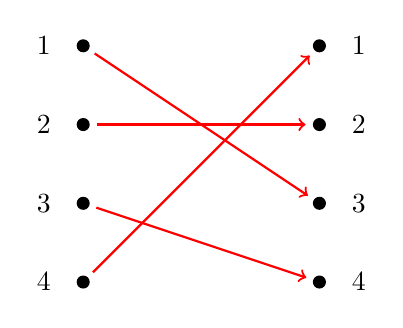
\begin{tikzpicture}
  \filldraw[black] (-1.5,0) circle (.5ex) {};
  \filldraw[black] (-1.5,1) circle (.5ex) {};
  \filldraw[black] (-1.5,2) circle (.5ex) {};
  \filldraw[black] (-1.5,3) circle (.5ex) {};
  \node at (-2, 0) {$4$};
  \node at (-2, 1) {$3$};
  \node at (-2, 2) {$2$};
  \node at (-2, 3) {$1$};

  \filldraw[black] (1.5,0) circle (.5ex) {};
  \filldraw[black] (1.5,1) circle (.5ex) {};
  \filldraw[black] (1.5,2) circle (.5ex) {};
  \filldraw[black] (1.5,3) circle (.5ex) {};
  \node at (2, 0) {$4$};
  \node at (2, 1) {$3$};
  \node at (2, 2) {$2$};
  \node at (2, 3) {$1$};

  \draw[thick,red,->,shorten <=5pt,shorten >=5pt] (-1.5, 3) -- (1.5, 1);
  \draw[thick,red,->,shorten <=5pt,shorten >=5pt] (-1.5, 2) -- (1.5, 2);
  \draw[thick,red,->,shorten <=5pt,shorten >=5pt] (-1.5, 1) -- (1.5, 0);
  \draw[thick,red,->,shorten <=5pt,shorten >=5pt] (-1.5, 0) -- (1.5, 3);
 \end{tikzpicture}
 \label{fig:permutace-jako-sipky}
 \caption{Permutace $\clr{\sigma}$ zakreslená šipkami.}
\end{figure}

Ačkoli je tento způsob zápisu intuitivní a podporuje představu permutace jako
\uv{proházení} prvků na množině, mnohem více se používá tzv. zápis v cyklech.
Důvody jsou primárně formální; z cyklického zápisu se velmi snadno totiž pozná,
jak \uv{řád} permutace, tak její rozložení na \uv{transpozi\-ce}. Oba pojmy
definujeme a vysvětlíme později.

Jelikož permutace jsou bijekce z množiny do téže množiny, můžeme vždy začít v
nějakém libovolné prvku a pokračovat po šipkách, dokud se nedostaneme opět na
ten samý prvek. Tento přístup formalizuje právě zápis do cyklů. Například
zápis permutace $\clr{\sigma} = (3\;2\;4\;1)$ do cyklů by vypadal takto:
\begin{figure}[h]
 \centering
 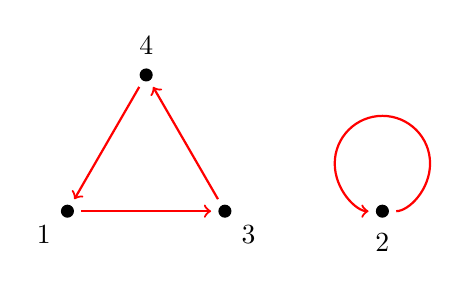
\begin{tikzpicture}
  \filldraw[black] (-1,0) circle (.5ex) {};
  \filldraw[black] (1,0) circle (.5ex) {};
  \filldraw[black] (0,1.73) circle (.5ex) {};

  \node at (-1.3, -0.3) {$1$};
  \node at (1.3, -0.3) {$3$};
  \node at (0, 2.1) {$4$};

  \filldraw[black] (3,0) circle (.5ex) {};
  \node at (3, -0.4) {$2$};

  \draw[thick,red,->,shorten <=5pt,shorten >=5pt] (-1, 0) -- (1, 0);
  \draw[thick,red,->,shorten <=5pt,shorten >=5pt] (1, 0) -- (0, 1.73);
  \draw[thick,red,->,shorten <=5pt,shorten >=5pt] (0, 1.73) -- (-1, 0);
  \draw[thick,red,->,shorten <=5pt,shorten >=5pt] (3, 0) arc (-90:270:4ex);
 \end{tikzpicture}
 \label{fig:permutace-jako-cyklus}
 \caption{Zápis permutace $\clr{\sigma}$ do cyklů.}
\end{figure}

Jak si asi dovedete představit, tento zápis znamená, že permutace $\clr{\sigma}$
pošle $1$ na $3$, pak $3$ na $4$ a nakonec $4$ na $1$. Tedy, po třech
\uv{iteracích} permutace $\clr{\sigma}$ se dostaneme z prvku $1$ opět do prvku
$1$. Smyčka nad $2$ samozřejmě znamená, že $2$ se zobrazuje opět na $2$.

Zápis na \hyperref[fig:permutace-jako-cyklus]{obrázku výše} je evidentně dosti
neúsporný, a v textu tudíž těžko použitelný. Obvykle se taková permutace zapíše
jako $\sigma = (134)(2)$. Tedy, jednotlivé cykly jsou odděleny závorkami a šipky
v cyklech vedou zleva doprava, případně z posledního prvku zpět na první.

Konečně, smyčky (tj. zobrazení prvku na sebe sama) se z cyklického zápisu běžně
vynechávají. Svoji oblíbenou permutaci $\sigma = (134)(2)$ můžeme proto úplně
nejúsporněji zapsat jako $\sigma = (134)$. Zápis permutací v cyklech budeme
odteď využívat výhradně.

\begin{warning}
 Zápis permutace pomocí cyklů \textbf{není jednoznačný}. Je to pro to, že u
 daného cyklu nelze říct, kde \uv{končí} a kde \uv{začíná}. Důležité je pouze
 pořadí prvků. Permutace $(134), (341)$ a $(413)$ jsou tudíž jedna a ta samá.
\end{warning}

\subsubsection{Skládání permutací}
\label{sssec:skladani-permutaci}

Jelikož permutace jsou speciálně zobrazení, dají se pochopitelně skládat. Navíc,
protože doména i kodoména každé permutace na $X$ je právě množina $X$, mohu je
skládat v libovolném pořadí a libovolném množství.

Na výpočet složení dvou permutací $\sigma,\tau \in S_X$ není myslím žádný
vyloženě snadný postup. Člověk se musí zkrátka v cyklickém zápisu dočíst, kam
posílá první permutace daný prvek, a kam zase druhá permutace posílá obraz
tohoto prvku.

\begin{example}
 Ať $X = \{1,2,3,4\}$ a $\sigma,\tau \in S_X, \sigma = (134), \tau = (14)(23)$.
 Pak
 \[
  \sigma\tau = (243),
 \]
 protože $\tau$ pošle $1$ na $4$ a $\sigma$ pošle $4$ na $1$, tedy  $\sigma\tau$
 pošle $1$ na $1$. Podobně pro ostatní prvky. V šipkách složení $\sigma\tau$ 
 vypadá takto:
 \begin{figure}[H]
  \centering
  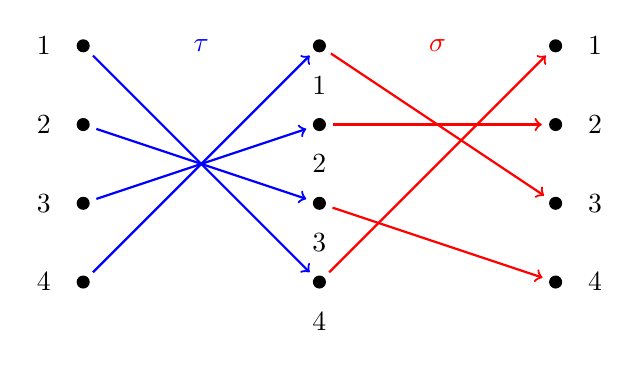
\begin{tikzpicture}
   \filldraw[black] (-1.5,0) circle (.5ex) {};
   \filldraw[black] (-1.5,1) circle (.5ex) {};
   \filldraw[black] (-1.5,2) circle (.5ex) {};
   \filldraw[black] (-1.5,3) circle (.5ex) {};
   \node at (-2, 0) {$4$};
   \node at (-2, 1) {$3$};
   \node at (-2, 2) {$2$};
   \node at (-2, 3) {$1$};

   \filldraw[black] (1.5,0) circle (.5ex) {};
   \filldraw[black] (1.5,1) circle (.5ex) {};
   \filldraw[black] (1.5,2) circle (.5ex) {};
   \filldraw[black] (1.5,3) circle (.5ex) {};
   \node at (1.5, -0.5) {$4$};
   \node at (1.5, 0.5) {$3$};
   \node at (1.5, 1.5) {$2$};
   \node at (1.5, 2.5) {$1$};

   \filldraw[black] (4.5,0) circle (.5ex) {};
   \filldraw[black] (4.5,1) circle (.5ex) {};
   \filldraw[black] (4.5,2) circle (.5ex) {};
   \filldraw[black] (4.5,3) circle (.5ex) {};
   \node at (5, 0) {$4$};
   \node at (5, 1) {$3$};
   \node at (5, 2) {$2$};
   \node at (5, 3) {$1$};

   \draw[thick,red,->,shorten <=5pt,shorten >=5pt] (1.5, 3) -- (4.5, 1);
   \draw[thick,red,->,shorten <=5pt,shorten >=5pt] (1.5, 1) -- (4.5, 0);
   \draw[thick,red,->,shorten <=5pt,shorten >=5pt] (1.5, 0) -- (4.5, 3);
   \draw[thick,red,->,shorten <=5pt,shorten >=5pt] (1.5, 2) -- (4.5, 2);

   \draw[thick,blue,->,shorten <=5pt,shorten >=5pt] (-1.5, 3) -- (1.5, 0);
   \draw[thick,blue,->,shorten <=5pt,shorten >=5pt] (-1.5, 0) -- (1.5, 3);
   \draw[thick,blue,->,shorten <=5pt,shorten >=5pt] (-1.5, 2) -- (1.5, 1);
   \draw[thick,blue,->,shorten <=5pt,shorten >=5pt] (-1.5, 1) -- (1.5, 2);

   \node[red] at (3, 3) {$\sigma$};
   \node[blue] at (0, 3) {$\tau$};
  \end{tikzpicture}
  \label{fig:slozeni-permutaci-sipky}
  \caption{Složení permutací $\clr{\sigma}\clb{\tau}$ znázorněno v šipkách.}
 \end{figure}
 Všimněte si ale, že
 \[
  \tau\sigma = (123).
 \]
\end{example}
\begin{warning}
 Jak bylo vidno z předchozího příkladu, skládání permutací (jako obecně i
 relací) \textbf{není komutativní}. Dokonce platí, že pouze skládání permutace
 se sebou samou je komutativní, čili jsou-li $\sigma,\tau \in S_X$, pak
 \[
  \sigma\tau = \tau\sigma \implies \tau = \sigma
 \]
 za předpokladu, že $\# X \geq 3$.
\end{warning}

Nyní si konečně povíme, co znamená \uv{řád} permutace a že každou permutaci lze
rozložit na \uv{transpozice}.

Když $\sigma = c_1c_2\cdots c_n$ je rozklad permutace $\sigma \in S_X$ na cykly
$c_1,c_2,\ldots,c_n$, pak \emph{délkou cyklu} $c_i$ myslíme počet prvků množiny
$X$, které se v něm vyskytují. Tedy, např. délka cyklu $(1324)$ je $4$ a délka
cyklu $(457)$ je $3$.

\begin{definition}[Transpozice]
\label{def:transpozice}
 Permutace $\sigma \in S_X$ se nazývá \emph{transpozice}, když obsahuje právě
 jeden cyklus délky $2$. Lidsky řečeno, transpozice jsou přesně ty permutace,
 které prohazují dva prvky.
\end{definition}

Možná trochu překvapivý výsledek ohledně permutací je, že každou permutaci lze
napsat jako složení transpozic. Navíc je algoritmus velmi přímočarý -- stačí
zkrátka každý cyklus délky $k$ rozložit na $k - 1$ transpozic tak, že každý
\uv{vnitřní} prvek cyklu zdvojíme. Zformulujeme si tvrzení a ukážeme si
algoritmus na příkladě.

\begin{claim}[Rozklad na transpozice]
 Ať $\sigma \in S_X$ a $\# X \geq 2$ (jinak bychom neměli dva prvky k
 prohození). Pak existují transpozice $\tau_1,\ldots,\tau_n$ takové, že
 \[
  \sigma = \tau_1\tau_2\cdots \tau_n.
 \]
 Navíc, počet transpozic v rozkladu $\sigma$ je určen jednoznačně.
\end{claim}
\begin{proof}
 Formální. Vynechám. Ideu si ukážeme na příkladě.
\end{proof}

\begin{example}
 Rozložíme permutaci $\sigma = (1342)(576)$ na transpozice. Každý cyklus vlastně
 rozdělíme na cykly délky dva (což jsou vlastně transpozice) zdvojením každého
 vnitřního prvku. Tedy, cyklus $(576)$ se rozdělí na transpozice $(57)$ a $(76)$
 a cyklus  $(1342)$ se rozdělí na $(13)$, $(34)$ a $(42)$. Pak dostaneme
 (\textbf{pozor na pořadí!})
 \[
  \sigma = (13) \circ (34) \circ (42) \circ (57) \circ (76),
 \]
 což je rozklad $\sigma$ na transpozice. Na
 \hyperref[fig:rozklad-na-transpozice]{obrázku} vidíte znázornění aplikace
 permutace $\sigma$ na množinu $\{1,\ldots,7\}$ a postupnou aplikaci příslušných
 transpozic.
 \begin{figure}[H]
  \centering
  \begin{tikzcd}
   1 \; 2 \; 3 \; 4 \; 5 \; 6 \; 7 \ar[ddddd, "\sigma = (1342)(576)"'] & 1 \; 2 \; 3 \; 4 \; 5 \; 6 \; 7 \arrow[d, "(76)"] \\
   & 1 \; 2 \; 3 \; 4 \; 5 \; 7 \; 6 \arrow[d, "(57)"] \\
   & 1 \; 2 \; 3 \; 4 \; 7 \; 5 \; 6 \ar[d, "(42)"] \\
   & 1 \; 4 \; 3 \; 2 \; 7 \; 5 \; 6 \ar[d, "(34)"] \\
   & 1 \; 3 \; 4 \; 2 \; 7 \; 5 \; 6 \ar[d, "(13)"] \\
   3 \; 1 \; 4 \; 2 \; 7 \; 5 \; 6 & 3 \; 1 \; 4 \; 2 \; 7 \; 5 \; 6
  \end{tikzcd}
  \label{fig:rozklad-na-transpozice}
  \caption{Znázornění rozkladu permutace $\sigma$ na transpozice.}
 \end{figure}
\end{example}

\begin{definition}[Sudá/lichá permutace]
\label{def:suda/licha-permutace}
 Permutaci $\sigma \in S_X$ nazveme \emph{sudou}, když její rozklad na
 transpozice obsahuje sudý počet transpozic. Jinak ji nazveme \emph{lichou}.
\end{definition}

Poslední zajímavý výsledek o permutacích, který zmíníme, říká, že když jednu
permutaci složím samu se sebou dostatečněkrát, dostanu identické zobrazení na
$X$. Počtu složení se formálně říká \uv{řád} permutace.

\begin{definition}[Řád permutace]
\label{def:rad-permutace}
 Mějme $\sigma \in S_X$. Přirozené nenulové číslo ${k \in \N}$ nazveme
 \emph{řádem} permutace $\sigma$, když
 \[
  \sigma^{k} = \mathds{1}_X.
 \]
 Řád permutace značíme $\ord \sigma$ (z angl. \textbf{ord}er).
\end{definition}

Na konec sekce si rozmyslíme, že každá permutace má konečný řád a jak ho
počítat. Uvažme třeba permutaci $\sigma = (143)$. Tahle permutace posílá $1$ na
$4$, $4$ na $3$ a $3$ zpět na $1$. To ovšem znamená, že když ji \uv{zopakuji}
třikrát za sebou, dostanu se rovnou z $1$ na $1$. Vskutku, můžete si ověřit, že
\[
 \sigma^3 = (143) \circ (143) \circ (143) = \mathds{1}_{\{1,2,3,4\}}.
\]
Tento pohled napovídá, že když cyklus délky $k$ zopakuji $k$-krát, zobrazím
všechny prvky v tomto cyklu na ony samé.

Co když mám ale permutaci složenou z cyklů různých délek, jako třeba
$(143)(25)$? No, cyklus $(143)$ musím zopakovat třikrát a cyklus $(25)$ dvakrát.
Když ale tuto permutaci třikrát zopakuji, nedostanu identické zobrazení, protože
cyklus $(25)$ zopakovaný třikrát je zase $(25)$. Když se zamyslíme, zjistíme, že
abych dostal z permutace identické zobrazení, musím ji opakovat právě tolikrát,
kolik je nejmenší společný násobek délek jejích cyklů, aby se každý cyklus
zopakoval nějakým násobkem své délky. Zformulujeme si tento fakt jako tvrzení,
ale dokazovat ho nebudeme, protože důkaz je otravně formální.

\begin{claim}[O řádu permutace]
 Ať $\sigma \in S_X$ a
 \[
  \sigma = c_1c_2\cdots c_n
 \]
 je zápis $\sigma$ v cyklech $c_1,\ldots,c_n$. Označme $d_i$ délku cyklu $c_i$ 
 pro každé $i \leq n$. Pak
 \[
  \ord \sigma = \mathrm{lcm}(d_1,\ldots,d_n),
 \]
 kde $\mathrm{lcm}$ (z angl. \textbf{l}east \textbf{c}ommon \textbf{m}ultiple)
 značí nejmenší společný násobek.
\end{claim}

Myslím, že tohle tvrzení je pěkným příkladem přirozeného avšak poměrně silného
tvrzení. Kdybyste nevěděli nic o permutacích a řekl bych vám, že máte dokázat
fakt, že když bijekci na konečné množině složím samu se sebou hodněkrát, dostanu
identické zobrazení, asi byste se zapotili.

\subsection{Problém sta vězňů}
\label{sssec:problem-sta-veznu}

Za sedmero horami a sedmero řekami, byla nebyla kdysi jedna věznice, ve které
bylo žilo a živořilo sto vězňů. Její dozorce, chor a zchřadl, matematik řemeslem
a krutovládce povahou, jednoho jitra rozhodl, že vězně propustí -- buď do světa,
nebo až do toho příštího.

Vyklidiv vězeňskou jídelnu, postavil zde sto dřevěných stolic nesoucích sto
papírových obálek. Mezi obálky rozloučil sto kamení, v každém toporně vyryto
různé číslo od jedné do sta.

Rozkázav vězně seřaditi před jídelnu, přičlenil každému rovněž různé číslo od
jedné do sta, v pořadí, kterak stáli. Vězni měli po řadě postoupit do jídelny a
otevřít padesát obálek. Našli-liž mezi nimi kámen zračící jejich číslo, vrátili
jej zpět a směli opustit jídelnu opačným východem.

Podmínka propuštění děla, že každý vězeň musí v jedné z padesáti obálek, které
otevřel, zřít své číslo. Pokud byť i jeden vězeň své číslo neobjeví, celé těleso
vězňů bude kvapně popraveno.

Asi není těžké si rozmyslet, že tohle je úloha na permutace. Pořadí, v jakém
jsou umístěny stolice, můžeme vnímat jako množinu přirozených čísel
$\{1,\ldots,100\}$ a rozmístění kamenů do obálek jako jednu její náhodně
zvolenou permutaci. Tedy, to, že v obálce číslo $6$ je kámen s číslem $23$
znamená, že tato permutace posílá prvek $6$ na prvek $23$.

Pokud by vězni vybírali obálky k otevření náhodně, pak má každý z nich na
nalezení kamene se svým číslem šanci přesně $1 / 2$. Protože tahle situace se má
opakovat stokrát po sobě, šance, že všichni najdou tímto způsobem své číslo, je
$(1 / 2)^{100}$, tedy $1$ ku $1 267 650 600 228 229 401 496 703 205 376$ -- čili
pořád větší, než že si MŠMT všimne, že existují počítače -- ale přesto malá.

My tvrdíme, že ve skutečnosti existuje strategie, která umožní vězňům uniknout
poslednímu dechu s šancí větší než 30 \%. Navíc je velmi přímočará. Stačí, aby
každý vězeň otevíral obálky v pořadí, které určují kameny v nich obsažené.
Konkrétně, každý vězeň otevře jako první obálku na stolici se stejným pořadím,
jako je to jeho. Další otevře obálku na stolici s pořadím, které odpovídá číslu
na kameni v obálce, kterou právě otevřel. Takhle pokračuje, dokud nenajde své
číslo, nebo dokud neprojde padesát různých obálek.

Ilustrujme si postup na příkladě. Do jídelny vstoupí vězeň s číslem $11$. Otevře
obálku číslo $11$ a najde v ní kámen s číslem $34$. Dále otevře obálku s číslem
$34$, v níž je číslo $77$. Ještě jednou, v obálce číslo $77$ najde číslo $5$. V
obálce číslo $5$ najde kámen s číslem $97$. A nakonec -- Ejhle! -- v obálce
číslo $97$ najde kámen se svým číslem -- $11$.

Označme permutaci určenou čísly na kamenech v obálkách třeba $\kappa$ (jako
\textbf{k}ámen). Situace v předchozím odstavci znamená, že v $\kappa$ existuje
cyklus
\begin{center}
 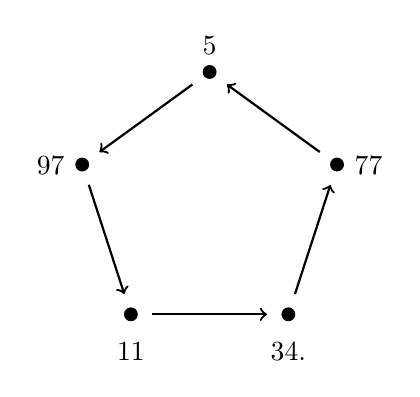
\begin{tikzpicture}
  \node[circle,fill=black,inner sep=0pt,minimum
  size=5pt,label={[yshift=-0.8cm]$11$}] (a) at (0,0) {};
  \path (a) ++(0:2) node [circle,fill=black,inner sep=0pt,minimum
  size=5pt,label={[yshift=-0.8cm]$34$.}] (b) {};
  \path (b) ++(72:2) node [circle,fill=black,inner sep=0pt,minimum
  size=5pt,label={[shift={(0.4cm, -0.35cm)}]$77$}] (c) {};
  \path (c) ++(144:2) node [circle,fill=black,inner sep=0pt,minimum
  size=5pt,label={[shift={(0cm, 0cm)}]$5$}] (d) {};
  \path (d) ++(216:2) node [circle,fill=black,inner sep=0pt,minimum
  size=5pt,label={[shift={(-0.4cm, -0.35cm)}]$97$}] (e) {};

  \draw[thick,->,shorten <=5pt,shorten >=5pt] (a) -- (b);
  \draw[thick,->,shorten <=5pt,shorten >=5pt] (b) -- (c);
  \draw[thick,->,shorten <=5pt,shorten >=5pt] (c) -- (d);
  \draw[thick,->,shorten <=5pt,shorten >=5pt] (d) -- (e);
  \draw[thick,->,shorten <=5pt,shorten >=5pt] (e) -- (a);
 \end{tikzpicture}
\end{center}

Nyní už si můžeme rozmyslet, za jaké podmínky objeví všichni vězni obálku s
kamenem svého čísla. V moment, kdy vězeň otevře první obálku, dostane se tím do
jednoho konkrétního cyklu permutace $\kappa$. Podle dané strategie bude tento
cyklus sledovat až do konce. Pokud je délka daného cyklu třeba $d$, pak v
moment, kdy otevře tento vězeň svoji $d$-tou obálku, bude v ní kámen s jeho
číslem. Samozřejmě, podmínka propuštění říkala, že každý vězeň smí otevřít
maximálně $50$ obálek. Protože každý vězeň má přiřazeno jiné, určitě čísla všech
vězňů dohromady vyčerpají všechny cykly permutace $\kappa$. To znamená, že
všichni vězni najdou svoje číslo tímto postupem jedině v případě, \textbf{kdy
permutace $\kappa$ neobsahuje cyklus délky větší než 50}. Zformulujeme si to
jako pozorování.

\begin{observation}
 Problém sta vězňů má řešení (tedy všech sto vězňů bude propuštěno) právě tehdy,
 když permutace $\kappa$, určená čísly na kamenech v obálkách, neobsahuje cyklus
 délky větší než $50$.
\end{observation}

Abychom spočítali šanci vězňů na úspěch, zbývá nám umět spočítat počet všech
takových permutací, tj. permutací s cykly délky maximálně $50$.

Ať $X \coloneqq \{1,\ldots,100\}$. Bude výhodnější řešit opačný problém, tedy
hledat počet permutací s cyklem délky aspoň $51$, protože (vzhledem k tomu, že
množina $X$ má $100$ prvků), takový cyklus tam může být nejvýše jeden.

Ať $C_n(S_X)$ značí počet všech permutací na $X$ s aspoň jedním cyklem délky
$n$. Jak jsme právě řekli, pro $n \geq 51$ může mít libovolná permutace takový
cyklus jenom jeden. Dále je zřejmé, že počet všech permutací s cyklem délky
\emph{aspoň} $51$ spočtu tak, že sečtu počty permutací s cyklem délky $n$ pro
všechna $n$ od $51$ do $100$. Když $C_{ \geq 51}(S_X)$ značí počet permutací s
cyklem délky aspoň $51$, máme
\[
 C_{ \geq 51}(S_X) = \sum_{n=51}^{100} C_n(S_X). 
\]

Spočítáme $C_n(S_X)$ pro $n \geq 51$. Abychom určili permutace s cyklem délky
$n$, musíme zvolit $n$ z těch $100$ čísel, která se v cyklu objeví. Počet
způsobů, jak zvolit $n$ čísel ze $100$ je $\binom{100}{n}$ (vizte sekci o
kombinačních číslech). %TODO
Čísla v tomto cyklu mohou být uspořádána $n!$ způsoby. \textbf{Ovšem, pozor!}
Nezapomeňte, že uvnitř cyklu mohu čísla posouvat a cyklus tím nechat stejný.
Protože mám v cyklu $n$ čísel, dělá to dohromady $n$ možných posunutí. Tedy mám
\[
 \frac{\binom{100}{n}n!}{n} = \binom{100}{n}(n-1)!
\]
různých způsobů, jak zvolit cyklus délky $n$.

Konečně, zbývající čísla (tedy ta mimo ten cyklus) můžu přeuspořádat $(100-n)!$
způsoby. Celkem, počet všech permutací s cyklem délky $n$ pro $n \geq 51$ je
\[
 C_n(S_X) = \binom{100}{n}(n-1)!(100-n)!.
\]
Je na čase završit výpočet. Všech možných permutací na $100$ číslech je $100!$.
Počet všech permutací s cyklem délky aspoň $51$ je $C_{\geq 51}(S_X)$. Čili šance,
že náhodně vybraná permutace na $100$ číslech \textbf{obsahuje} cyklus délky
větší než $50$ je
\[
 \frac{C_{ \geq 51}(S_X)}{100!} = \frac{\sum_{n=51}^{100} C_n(S_X)}{100!} =
 \frac{\sum_{n=51}^{100} \binom{100}{n}(n-1)!(100-n)!}{100!} \approx 0.688,
\]
čili $68,8~\%$. To ovšem znamená, že šance, že náhodná permutace
\textbf{neobsahuje} cyklus délky větší než $50$ je přibližně $1 - 0.688 =
0.312$. Takže při využití této strategie mají vězni přibližně  $31.2~\%$ na
přežití. O něco lepší než náhodné zkoušení.

\begin{exercise}
 Spočtěte složení $\sigma\tau$ a $\tau\sigma$, když
 \begin{enumerate}[topsep=0pt,label=(\arabic*)]
  \item $\sigma = (143)(26), \tau = (146)(253)$,
  \item $\sigma = (14)(25)(36), \tau = (123456)$,
  \item $\sigma = (145)(263), \tau = (154)(236)$.
 \end{enumerate}
\end{exercise}

\begin{exercise}
 Určete řád permutace $\sigma$, kde
 \begin{enumerate}[label=(\arabic*),topsep=0pt]
  \item $\sigma = (1345)$,
  \item $\sigma = (1346)(28)(579)$.
 \end{enumerate}
\end{exercise}

\begin{exercise}[těžké]
 Určete číslo $C_n(S_X)$, kde $\# X = 100$ a $n \leq 50$, tedy počet všech
 permutací na $100$ číslech s aspoň jedním cyklem délky menší nebo rovné
 $50$.
\end{exercise}

\begin{exercise}
 Ať $\sigma \in S_n$, tedy $\sigma$ je permutace množiny $\{1,\ldots,n\}$.
 Řekneme, že $\sigma$ \emph{invertuje} dvojici $(i,j)$, kde $i,j \in
 \{1,\ldots,n\}$, když $i<j$, ale $\sigma(i)>\sigma(j)$.

 Definujme
  \[
   I(\sigma) \coloneqq \{(i,j) \in \{1,\ldots,n\}^2 \mid \sigma \text{ invertuje
   } (i,j)\},
 \]
 čili $I(\sigma)$ je množina všech dvojic $(i,j)$, které $\sigma$ invertuje.
 Uvědomme si, že $I(\sigma)$ je podmnožinou $\{1,\ldots,n\}^2$, čili relací na
 $\{1,\ldots,n\}$.
 \begin{enumerate}[label=(\arabic*),topsep=0pt]
  \item Dokažte, že $I(\sigma)$ je transitivní relace na $\{1,\ldots,n\}$ pro
   každou permutaci $\sigma \in S_n$.
  \item* Navrhněte algoritmus, který pro danou permutaci $\sigma \in S_n$ spočte
   $\# I(\sigma)$.
  \item Spočtěte počet invertovaných dvojic, čili $\# I(\sigma)$, permutací
   $\sigma = (134)(579)(26)$.
 \end{enumerate}
\end{exercise}
